%Created with command:
%"/home/josh/Teaching/trunk/Utilities/makeexam" "Exam 2" "Please complete each problem.  Show all of your work even if you cannot obtain the correct answer.  You may use only a single sheet of letter sized paper for assistance." "../VHDL/Assessments/concurrent_statement.tex" "../VHDL/Assessments/process.tex" "../CombinationalDesign/Assessments/timing_read_write_ex.tex" "../Decoders/Assessments/2to4decoder.tex" "../XOR/Assessments/memory_parity_extended.tex" "../Encoders/Assessments/binary_encoder.tex" "../VHDL/Assessments/msi74x682.tex"
\documentclass{article}
\usepackage[T1]{fontenc}
\usepackage{arev}
\usepackage{longtable}
\usepackage[hmargin=2cm,vmargin=2cm]{geometry}
\usepackage{graphicx}
\usepackage{listings}
\setlength{\parindent}{0pt}
\title{Exam 2}
\date{}
\begin{document}
\maketitle
Please complete each problem.  Show all of your work, even if you cannot obtain the correct answer.  You may use only a single sheet of letter sized paper for assistance. (44 points total)
\begin{longtable}[l]{rp{17cm}}
%file: ../VHDL/Assessments/concurrent_statement.tex
1.&\begin{minipage}[t]{\linewidth}(2 pt) A colleague shows you the following VHDL code, which does not work as expected.  Briefly describe the problem with this architecture.
\lstset{language=VHDL}
\begin{lstlisting}
library ieee;
use ieee.std_logic_1164.all;

entity inverter is
    port (X: in std_logic;
          F: out std_logic);
end entity;

architecture inverter_arch of inverter is
begin
    X <= not X;
    F <= X;
end inverter_arch;
\end{lstlisting}

\vspace{6cm
}
\end{minipage}\\
\medskip
%file: ../VHDL/Assessments/process.tex
2.&\begin{minipage}[t]{\linewidth}(2 pt) Briefly describe the role of the sensitivity list in the VHDL process statement.

\vspace{6cm
}
\end{minipage}\\
\medskip
%file: ../CombinationalDesign/Assessments/timing_read_write_ex.tex
3.&\begin{minipage}[t]{\linewidth}(2 pt) You have been given the following timing diagram as part of the documentation for a circuit that you are reviewing.  Please explain a possible problem with the operation of this circuit.\\ \\
\begin{center}
  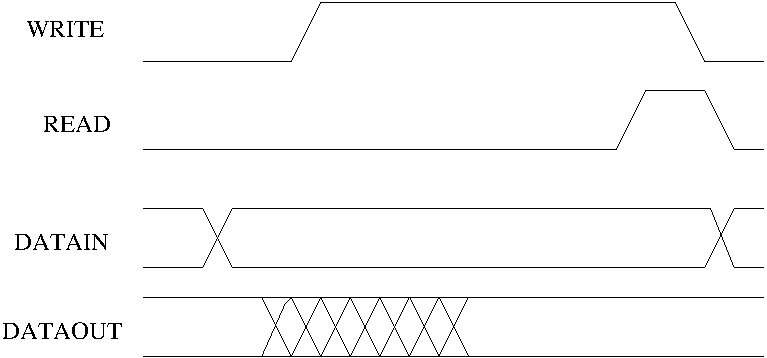
\includegraphics{../CombinationalDesign/Assessments/TimingDiagramReadWriteUnstableDataIn}
\end{center}

\vspace{6cm
}
\end{minipage}\\
\medskip
%file: ../Decoders/Assessments/2to4decoder.tex
4.&\begin{minipage}[t]{\linewidth}(10 pt) Using the following logic circuit (a) write a logic function for each output (Y0, Y1, Y2, and Y3) and (b) determine which common component this logic circuit represents.\\
\begin{center}
  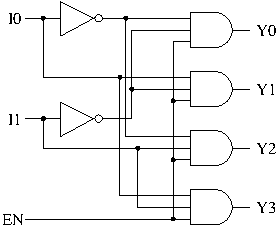
\includegraphics{../Decoders/Assessments/2to4BinaryDecoderLogic} \\
\end{center}

\vspace{8cm
}
\end{minipage}\\
\medskip
%file: ../XOR/Assessments/memory_parity_extended.tex
5.&\begin{minipage}[t]{\linewidth}(8 pt) You have been asked to extend the memory parity circuit to work with a 16 bit data bus.  Given the following schematic diagram, correctly connect the two areas in the dotted lines - the ERROR signal circuit and the PIN input to the memory.  You may need to use some additional logic gates.
\begin{center}
  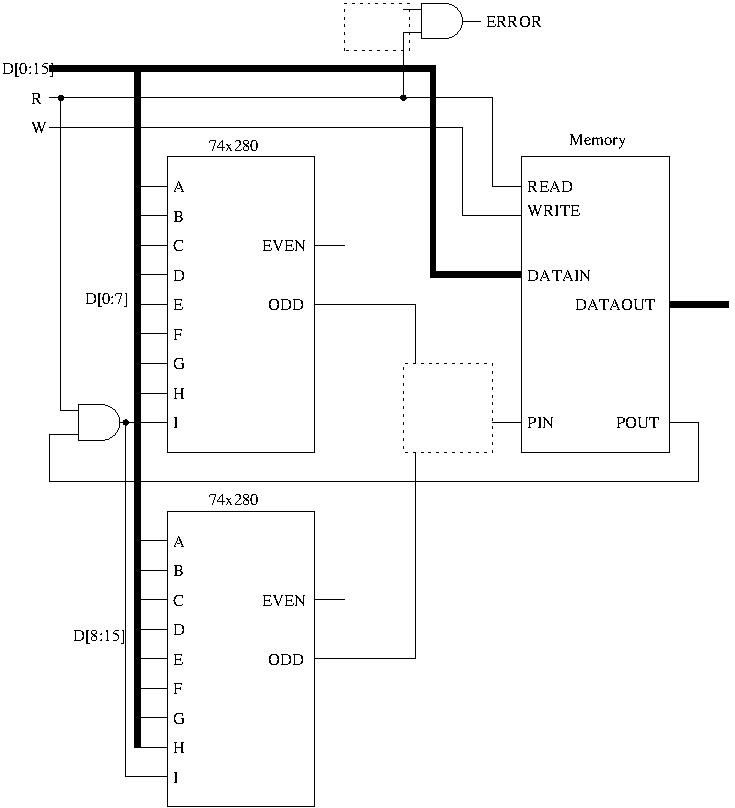
\includegraphics[scale=0.5]{../XOR/Assessments/MemoryCircuitParityExtended}
\end{center}

\vspace{6cm
}
\end{minipage}\\
\medskip
%file: ../Encoders/Assessments/binary_encoder.tex
6.&\begin{minipage}[t]{\linewidth}(10 pt) The following circuit diagram is an implementation of a 4-to-2 binary encoder.  Modify this implementation to create a 4-to-2 binary encoder that uses \textbf{only NAND gates}.  Make sure that the input and the output to your circuit are both active high.
\begin{center}
  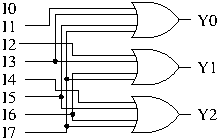
\includegraphics{../Encoders/Assessments/BinaryEncoderLogic}
\end{center}

\vspace{14cm
}
\end{minipage}\\
\medskip
%file: ../VHDL/Assessments/msi74x682.tex
7.&\begin{minipage}[t]{\linewidth}(10 pt) Using VHDL, write the architecture for a 74x682 comparator.  Use the entity provided below.  I will email you a test bench that you should use to validate your program.  You may use your text, examples from class, and even resources on from the Internet for this problem.  However, please \textbf{do not discuss the solution to this problem with other students in this class}.  Please email me your .vhd file by 6:00 AM Saturday, March 21.
\lstset{language=VHDL}
\begin{lstlisting}
entity msi74x682 is
    port (P: in std_logic_vector(7 downto 0);
          Q: in std_logic_vector(7 downto 0);
          PEQQ_L: out std_logic;
          PGTQ_L: out std_logic);
end msi74x682;
\end{lstlisting}

\vspace{2cm
}
\end{minipage}\\
\medskip
\end{longtable}
\end{document}